\documentclass[letterpaper,10pt]{article}
\usepackage[dvips]{graphicx}

\author{Eric Dutko \and Jason Grusauskas \and Michael Korman \and David Walluck}
\title{Description of the Adder System}

\begin{document}
\maketitle

\section{Introduction}

The goal of this project is to implement an online voting system that
is both secure and open. The openness of the system is important for
obtaining public confidence and public trust in the system.

The system will function by having a group of publicly known and
trusted authorities. An election can be initiated if a certain
predetermined and publicly known number of the trusted authorities log
in to the server and request an election. Requiring multiple
authorities creates confidence about the integrity of the election
(e.g., it is harder to bribe 100 ``trusted'' people than it is to
bribe one). Once the predetermined subset of authorities has logged
in, the server uses the keys of the authorities to create a public key
that will be used by the voters for the encryption of their votes.

Once this is done, the system moves into state 2. In state 2, the
authorities no longer have system control. The system now listens for
connections from voters.  

One important aspect of the openness of the system is that in the
voting stage the entire systems contents is viewable by voters,
authorities and the general public. Each voter is registered and
therefore has a given area set aside inside the server to house their
encrypted vote. Each voter encrypts and also computes a proof of
validity on the client side. The proof is necessary so that the server
and the public viewing the server know that the encrypted vote is a
valid one. By doing this on the client side the server never touches a
raw vote, only the encrypted vote--and therefore
indeterminable--string. Once the voting is complete the server
transitions into state 3, at which point it waits for the
predetermined number of authorities to log in again. Once the
predetermined authorities have logged back in, the server takes their
keys and uses them to run a summation of the encrypted strings. The
result is the total of votes. This process can also be verified by a
verification program.

This is just a brief overview of the way in which we would implement
this system. Of course, due to this being a ``short description'' the
complex encryption schemes and details of the system implementation
are excluded.

\section{Overview of Components}

\subsection{Web Server}

The Apache web server is running and is configured for secure
connections. Users can connect with a web browser over SSL and log in,
with authentication being performed directly with the database. Users
can also post messages directly to the database through a web
interface. These messages can be viewed by connecting directly to the
database with a public read-only account.

The protocol for communication with the CryptoServer is sufficiently
complete to allow for the above activities (i.e. authentication of
users and message submission). Most of the written protocol has been
implemented on both ends and is in the initial stages of testing.

\subsection{Encryption Library}

The encryption library (libadder) is the other main piece of the
system (aside from the Adder server). The encryption library contains
the ElGamal code, and links with a supporting library (e.g. GMP) which
provides underlying support for multi-precision integer arithmetic.

\subsection{CryptoServer}

The CryptoServer is written in C++, using the ACE networking library.
It is a multi-threaded server that dedicates one thread to each
connecting client. The server is responsible for accepting connections
from the Web server, and performing all database operations requested
by the Web server, such as user authentication, vote adding, etc.

The server uses the MySQL++ library to communicate with the MySQL
database. We are in the process of writing a wrapper around this
library, which encapsulates all of the database functionality we need.

The CryptoServer uses a local copy of libadder to perform all of its
cryptographic operations.

Currently, the CryptoServer is capable of authenticating users, and
adding votes to the database.

\subsection{Mozilla Plugin}

The plugin is currently for Mozilla (either x86 or PPC) only, but we
may create IE or Windows versions as time permits. The plugin controls
encryption on the client's computer using the same encryption library
as the server side. The plugin only exists as \emph{glue} between the
encryption library and the PHP code which has the ability to talk
directly to the Adder server.

When a user connects to the Adder home page for the first time, he
should say `Cancel' to the box asking him to search for a plugin
supporting mime type \texttt{application/adder}, and instead install
the plugin from the home page which contains a link to the XPI
(cross-platform) installer. The installer is a normal zip file
containing some JavaScript code in \texttt{install.js} which tells the
plugin where it should install to and can detect whether or not the
installation was successful. A single click and about a second are all
it takes to install the client software.

The plugin and the PHP code will communicate to pass any shared values
back and forth, such as the key(s), the user's vote/values, etc.
Currently this may be able to be done the same way that CGI usually
works.

The plug-in is written in C++, and uses a copy of the libadder library
to do local cryptographic operations (i.e. encryption of the choice).
It also uses XPCOM to communicate between JavaScript and C++, and
includes JavaScript helper functions for the PHP. XPCOM is Mozilla
technology that allows bi-directional scripting C++ to JavaScript or
JavaScript to C++. The plug-in exports JavaScript functions which are
callable from JavaScript within the HTML code that the PHP generates
such as encryptVote and createKeyPair, etc. The reason for
choosing Mozilla is that it allows both Windows and Linux versions.

\subsection{System Diagram}
Figure \ref{fig:diagram} shows a diagram of the entire system.

\begin{center}
  \begin{figure}
    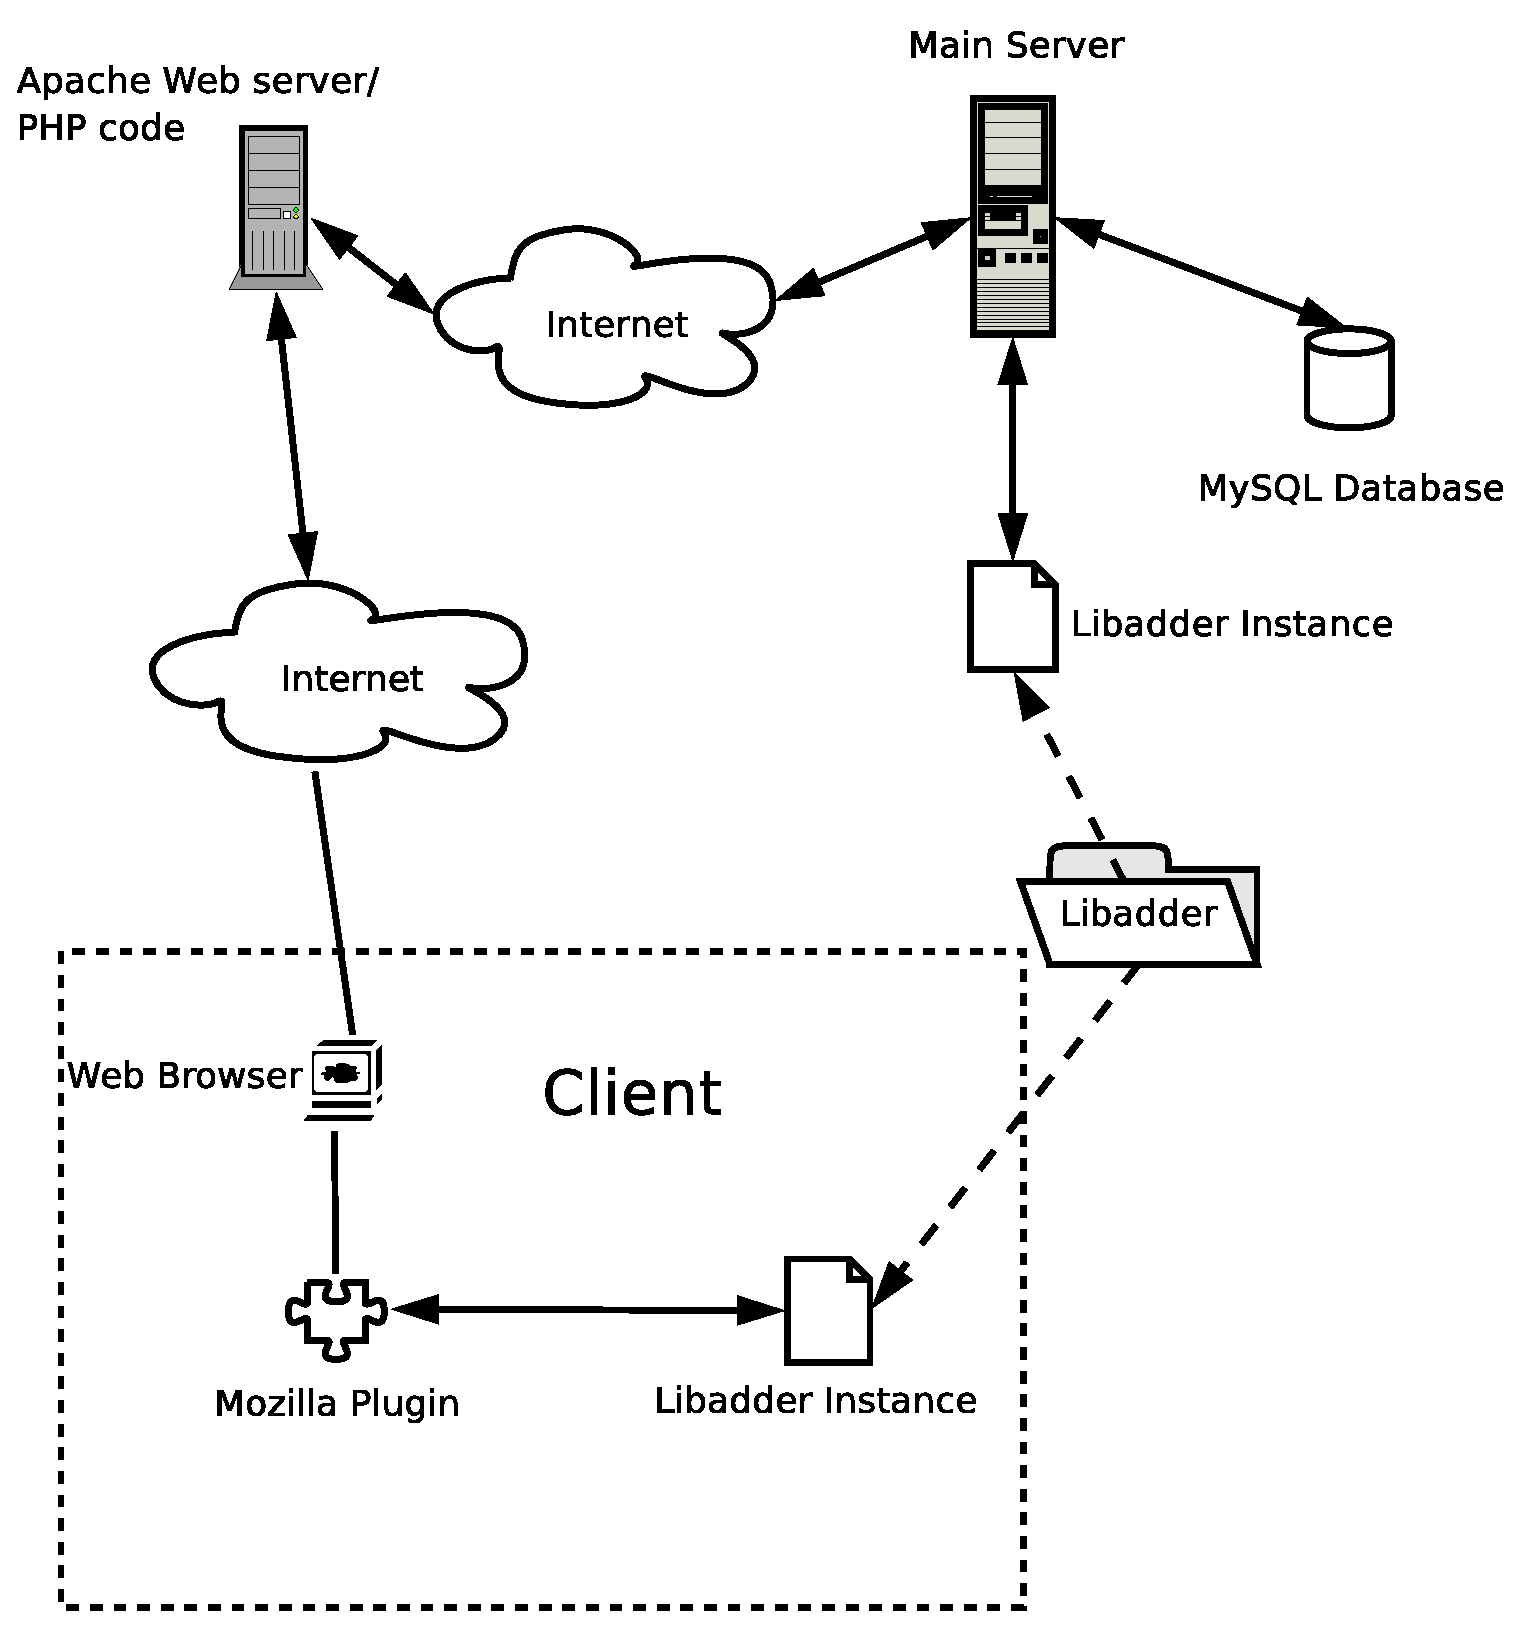
\includegraphics[scale=0.40]{diagram.eps}
    \caption{System diagram.}
    \label{fig:diagram}
  \end{figure}
\end{center}

\section{Design Alternatives}

For this project both the problem and the general specification of the
solution were well-defined. Professor Kiayias laid out an overview of
the total system, including specifics of all of the cryptographic
functionality. Thus, the design considerations left for our team
centered around how we should implement the system. In our planning
process, we considered a few different ways to lay out the system and
a few different distributions of the functionality among the
components before deciding on our current design.

The first design consideration we examined was deciding how users
would access our system. We considered a stand-alone client and
various ways of interacting via a Web server. Since a major part of the
project's goals was to produce a system that could be used as
universally as possible, we decided to allow users to access our
system via a Web browser. This eliminated any sort of stand-alone
client option. Once this decision was made, we wrestled for a while
with how we might accomplish this goal.

Because Web browsers are too limited to perform the type of encryption
and key-generation functions we needed, we concluded that we must
supplement the Web browser somehow. We considered creating a
scaled-down Web server with the necessary cryptographic functionality
that could run on the client's machine, acting as an interface to the
CryptoServer. We also considered creating a plugin which would perform
the necessary operations for the Web browser. While creating a plugin
required much more research and carried with it many unknowns, we chose
the benefit of a plugin's versatility and ease of use over the more
cumbersome miniaturized-Web server design.

Tied to this issue was the decision of how the server should be
implemented. For instance, a stand-alone client would have given us
much greater flexibility in implementing the server, but the benefits
to the end user of building a Web-accessible system were great enough
to trump the small savings in design and coding time. This left us
with three options for serving Web browser clients: 
\begin{enumerate}
\item Build our own Web server with the necessary cryptographic
  functionality.
\item Make use of an existing Web server such as Apache by building a
  module to extend it with our encryption functionality.
\item Use a Web server in combination with a scripting language such
  as PHP to act as an intermediary between the Web clients and our
  CryptoServer.
\end{enumerate}

We chose to make use of Apache and PHP as an intermediary for several
reasons. Constructing a Web server--even of limited scope and
capability--would have occupied a large portion of our design, coding,
and testing time. Apache is an open source Web server which has
already been tested and stabilized, and it is available for a large
number of platforms. Had we not made use of Apache, it is likely that
we would not have much more than a Web server completed by this time.

The choice to make a stand-alone server instead of an Apache plugin
was not such a clear-cut decision. An Apache module would have
simplified installation and use of the server. However, it would have
required more time and research in design, coding, and debugging.
Moreover, a bug in our code might result in the entire Web server
crashing--a serious problem if the Web server were running more than
just our system.

Implementing the server as a stand-alone program allowed us to avoid
the difficulties of an Apache module and avoid tying ourselves
directly to Apache. We found that PHP offered a very easy way to
communicate between the Web server and our CryptoServer, while still
allowing us to develop a communication protocol that could allow any
sort of client to interface directly with the CryptoServer. Of
course, the PHP also provided an simple channel for dynamically
creating Web pages with the appropriate data embedded for
communication to the client's browser plugin.

The final design decision was the inclusion of a database for
management of all of the CryptoServer's information. This allowed us
to make use of data storage and retrieval technology which is robust
and failsafe. It also allowed us to develop a permissions system at
the data-access level to add further protection against a compromised
server tampering with data. Finally, the database allowed us the
possibility of direct auditing of procedures by anyone in the world.
With a read-only account to the database made publicly available, the
possibilities for auditing are greatly expanded.

\section{Limitations and Future Extension Potentials}

As it stands, the project lacks several components necessary for a
complete system:

\begin{itemize}
\item Proofs of knowledge are needed to ensure that choices made by
  the client are valid. For example, in a 0/1 election, the client
  could vote 2, and this would count as two votes for 1.  The client
  must formulate a proof that it is voting one of the correct choices,
  and the server must validate this.  Proofs are important, since the
  server cannot read the clients vote directly, as it is encrypted.
  
\item Choices should be generalized to allow elections with more than
  two options.
  
\item Since our system is designed to be completely audit-able, it
  would be ideal to provide users with a sample program that actually
  performs the auditing.  This program would connect directly to the
  MySQL database, and perform various calculations to ensure that an
  election has not be tampered with in any way.
  
\item Currently, the CryptoServer does not automatically detect when
  elections are to be ended. In the configuration for a given
  procedure, a timeout is specified, but the server crashes when the
  timeout is reached.  Consequently, we require a user to manually end
  the election.  We believe that this problem is caused by a
  concurrency issue in the network library used by the server, and are
  investigating the matter.
  
\item The CryptoServer and the Web server should communicate with each
  other via SSL.  This would allow the two of them to communicate
  securely while located on separate machines. Currently, the client
  and the Web server do use SSL.
  
\item The CryptoServer should be made distributed, to increase fault
  tolerance (e.g., against denial-of-service attacks).
  
\item The protocol that the CryptoServer and Web server use should
  probably be redesigned.  It is very ad hoc at the moment, and should
  be formally defined. It is worth looking into using some form of XML
  for this.
  
\item We currently have functions to perform Radix-64
  encoding/decoding and ASCII armoring of all our cryptographic
  objects.  However, this functionality is not yet supported by the
  rest of the system, so it remains disabled. This is especially
  useful if we decide to use a binary format for the transfer of our
  objects over a network.
\end{itemize}

We do plan to fix all of these problems in the near future.
\end{document}
